\chapter{Converting Vector Spaces into Interpretable Representations}\label{Chapter3}
\section{Introduction}

%Why do this work? What is the value of this work?  How is this relevant to the readers interests?
%%Generally, what niche of interpretability are we trying to fill? Why? What's our motivation for this chapter? Why interpretable classifiers?


%What are some other interpretable representations? What are their advantages or disadvantages?
Distributional representations like vector spaces have the ability to represent semantic information spatially. Vector spaces built from a domain-specific corpus of text that represent this kind of information, also known as 'semantic spaces', are used, for instance, to represent items in recommender systems \cite{Vasile:2016:MPE:2959100.2959160,liang2016factorization,van2016learning}, to represent entities in semantic search engines \cite{DBLP:conf/sigir/JameelBS17,van2017structural}, or to represent examples in classification tasks \cite{DBLP:conf/iccv/DemirelCI17}. %Copied from CONLL paper.
One way to understand how a semantic space represents information is as a conceptual space \cite{Gardenfors2014}. In this space, we can understand domain entities, e.g. movies in a domain of IMDB movie reviews, to be represented as points, and domain properties to be in regions around these points. In figure \ref{ConceptualSpace}, we show an example conceptual space for movies. 


\begin{figure}[t]
	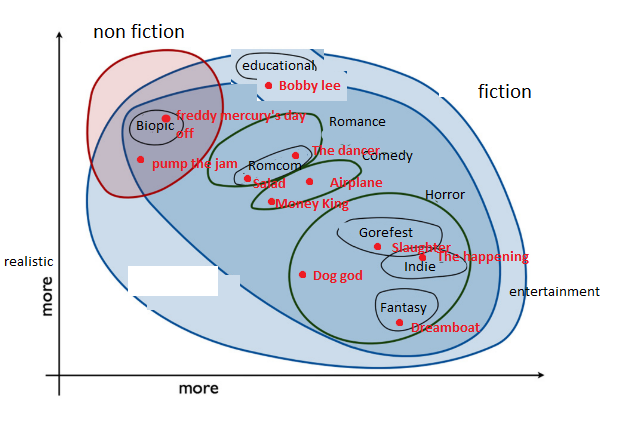
\includegraphics[width=\textwidth]{images/conceptualspace.png}
	\centering
	\caption{A conceptual space of movies, where regions correspond to properties and entities are points.}\label{ConceptualSpace}
\end{figure}

The success of these semantic spaces has lead many to investigate how the similarity-based structure can be converted into formal relationships. For example, in word-vectors (see Section \ref{WordVectors} for more) \cite{TomasMikolovWen-tauYih2013} found that "equivalent relations tended to correspond to parralel vector differences" \cite{Mitchell2015}, while \cite{Mitchell2015} discovered that by decomposing representations into orthogonal semantic and syntactic subspaces they were able to produce substantial improvements on various tasks.  %Copy pasted from this 

%%What is the previous work?
The semantic relation that we focus in on this paper are directions that correspond to salient features from the considered domain. %What is a direction
A direction is the orthogonal direction to a hyper plane that separates a term in a vector space. As the hyper plane separates entities, this means that the entities furthest along the hyper plane, at the end classified positively, are the entities we are most sure have the term we found the hyper plane for. To see an example of this, see \ref {LRHyperPlane} With this understanding, it becomes possible to induce a ranking of entities on the properties by finding the dot product of the entity points on the direction vector. 

These kind-of directions have been used in many different ways for different domains, For instance,  \cite{gupta2015distributional} found that features of countries, such as their GDP, fertility rate or even level of CO$_2$ emissions, can be predicted from word embeddings using a linear regression model. Similarly, in \cite{kim2013deriving} directions in word embeddings were found that correspond to adjectival scales (e.g.\ bad $<$ okay $<$ good $<$ excellent) while \cite{DBLP:conf/acl/RotheS16} found directions indicating lexical features such as the frequency of occurrence and polarity of words. 

%Finally, \cite{derracAIJ} found salient properties as direction vectors in a semantic space of entities (e.g. Movies in a domain of IMDB movie reviews), and labelled them with clusters of words (e.g. $p_1 = {Scary, Horror, Gore}, p_2 = {Funny, Laughter, Hilarious}$).  We show a toy example in Figure \ref{ToyDirection}. %Copied from CONLL 
By finding the dot product between entity points in the space and direction vectors, it is possible to induce a ranking of entities on those directions. In this chapter, we more deeply investigate the potential of direction vectors to rank entities on properties to form an interpretable representation. 

 In this thesis, we refer to these direction vectors as directions to convey the ordinal meaning, and directions as 'properties' if they are sufficiently salient in the space, e.g. In a domain of IMDB movie reviews where movies are entities, a direction on the word "The" would not be a property, but a direction on the word "Horror" would be. 

\begin{figure}[t]
	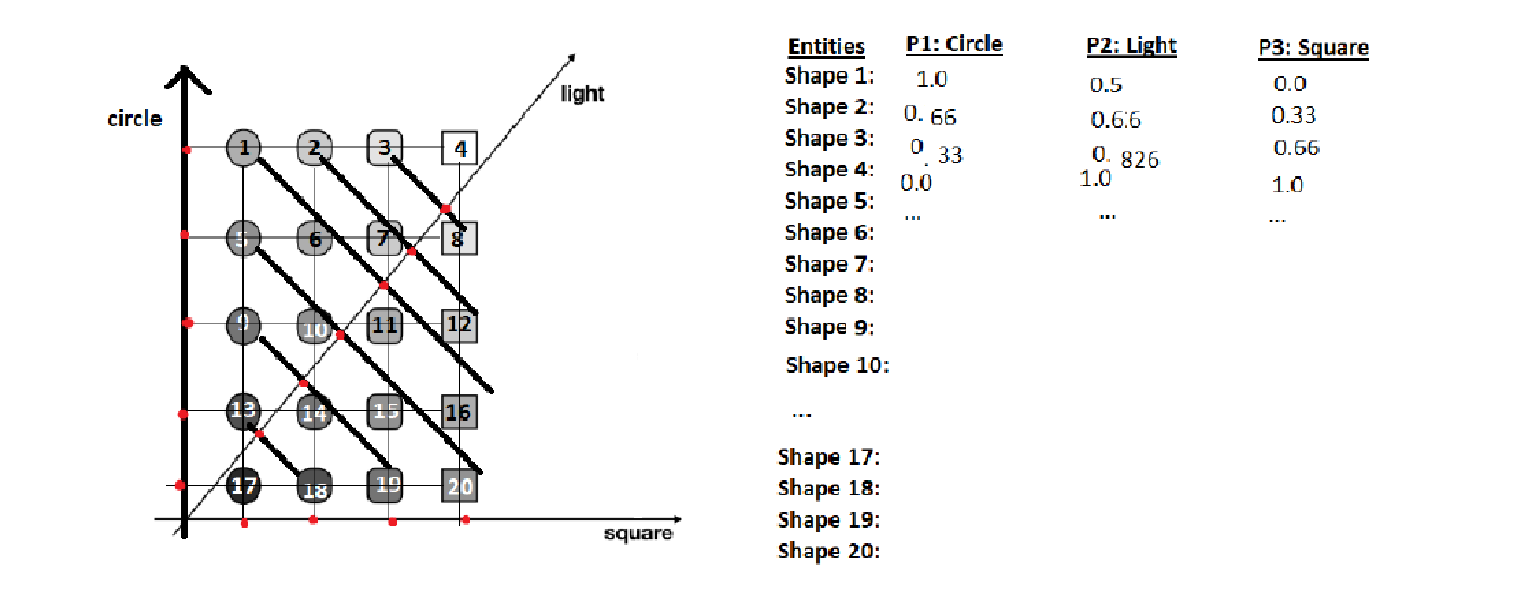
\includegraphics[width=\textwidth]{images/toydirections.png}
	\centering
	\caption{This figure shows a 2d toy space where entities are shapes and directions are properties. We demonstrate on the right the method to induce a ranking from the directions, in particular by using the dot-product of the entity point on the directions vector. In the same way for a more complex space, we can understand each entity point to be ranked on thousands of property directions, and the space to be much higher dimensionality.}\label{ToyDirection}
\end{figure}

 Such properties are useful in a wide variety of applications. The most immediate example is perhaps that they allow for a natural way to implement critique-based recommendation systems, where users can specify how their desired result should relate to a given set of suggestions \cite{viappiani2006preference}. For instance, \cite{Vig:2012:TGE:2362394.2362395} propose a movie recommendation system in which the user can specify that they want to see suggestions for movies that are ``similar to this one, but scarier''. If the property of being scary is adequately modelled as a direction in a semantic space of movies, such critiques can be addressed in a straightforward way. Similarly, in \cite{kovashka2012whittlesearch} a system was developed that can find ``shoes like these but shinier'', based on a semantic space representation that was derived from visual features. Semantic search systems can use such directions to interpret queries involving gradual and possibly ill-defined features, such as ``\emph{popular} holiday destinations in Europe'' \cite{DBLP:conf/sigir/JameelBS17}. While features such as popularity are typically not encoded in traditional knowledge bases, they can often be represented as semantic space directions.  %Copied from CONLL

%%What are the advantages, disadvantages of the previous work?

We demonstrate the effect of different filtering methods to find properties, the ability of different clustering methods to label properties, as well as the number and types of directions, for use in a low-depth interpretable linear classifier; a Decision Tree. In Figure \ref{IntroDecisionTree}, we demonstrate how depth could affect a Decision Tree that uses salient properties. These trees are not only evaluated quantitatively on key domain tasks, we also evaluate how interpretable the resulting rules are. This gives us a comprehensive idea of how we can use these rankings as an interpretable representation. By using a Decision Tree, we can identify salient properties - if we are able to construct a simple but high-scoring classifier for if a movie is a 'Comedy' using only our ranking of entities on the property $p = {"Funny", "Hilarious", "Laughing"}$ then we know that this property is salient. Although this is an extreme case, for more complex concepts, if we have salient properties that form the building blocks of this concept, then the model can be less complex and more general, two desirable properties for interpretable classifiers. 

\begin{figure}[t]
	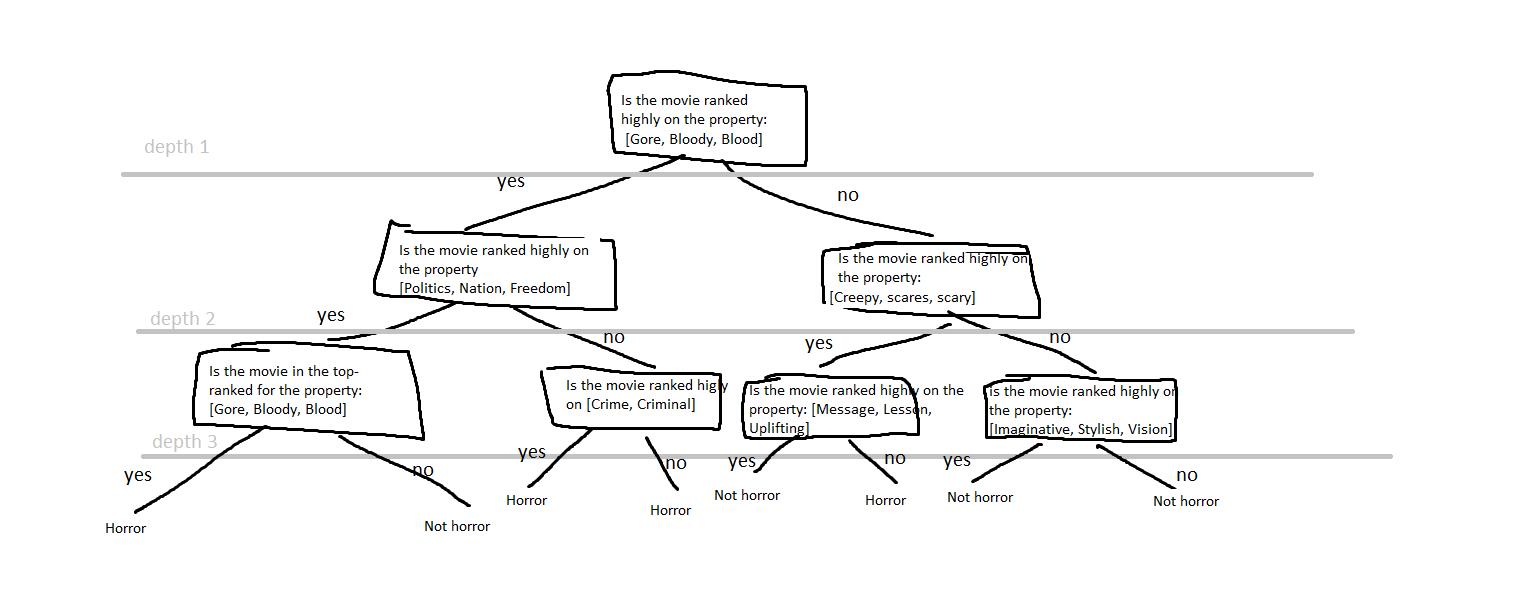
\includegraphics[width=\textwidth]{images/decisiontree.png}
	\centering
	\caption{This figure shows an example tree from one of our classifiers. Here, we can see that the model increases in complexity as it increases in depth. In this case, we end-up getting better F-score with just a depth-one tree, as the tree begins to overfit at depth three.  }\label{IntroDecisionTree}
\end{figure}

%%What is our contribution towards those disadvantages in this chapter?
 %"Decision Trees, Decision Tables and Textual descriptions of rules are logically equivalent in the sense that one type of representation can be automatically translated to another (albeit in a simpler or more complex form), while preserving the predictive behaviour of the original model"
% has many positive effects for its users, like lower response times \cite{Narayanan2018, Huysmans2011}, better question answering and confidence for logical problem questions \cite{Huysmans2011} and higher satisfaction \cite{Narayanan2018}.


%%What are some real world scenarios that you could see our work taking effect in?
In a case study by  \cite{Veale2017}, giving the business users the option between a model with higher classification score but more input variables and a lower classification score but less input variables resulted in more buy-in for system designers. By accurately representing salient concepts in the domain, we are also able to offer a similar option; less nodes in the decision tree in exchange for more accuracy. % Potentially this citation sucks


%How is the work evaluated? How can you justify the evaluation? 
%%What are some alternative interpretable classifiers? What are some approaches to interpretable classification?

%%How does our work fit into the niche of interpretable classifiers?

%%What kind of tasks are these interpretable classifiers usually on? How do we compare in terms of evaluation?

%%How does our evaluation of interpretability play into our idea of interpretability outlined in Chapter 1?

%How is the chapter going to play out? Whats going to happen?

This chapter continues as follows: We begin by describing the work related to this method, giving valuable context for the utility and potential of our approach. This is followed by an explanation of the method, including the variations we have adopted for our experimental work. We follow this with our qualitative experimentation, explaining how these variations affect the results, as well as the interpretability of the method, and we end with a quantitative analysis on how well we can represent domain knowledge using decision trees constrained to a limited depth.



\section{Related Work}
%Sparse word vectors
%Adapted to composition \cite{Fyshe2015}

%[ENTIRE SECTION COPY PASTED FROM PREVIOUS PAPER]
\textbf{Linear Classifiers}
Decision trees, linear SVM's, logistic regression, decision tables, IF Then rules.

What are the available options for interpretable linear classification?

How have each of these methods been measured or validated in the literature in regards to interpretability? How about application to real world situations?

\textbf{Non linear classifiers}
What non linear classifiers networks are interpretable? How have they done it? How have they measured it? How does it compare to a linear method?

\textit {Neural networks}Approximating w/linear model, Interpretable nodes/weights

\textit {Other Stuff}

\subsection{Interpretable Representations}


\subsection{Interpretable Classifiers}


There are two ways in which topic models can be used for document classification. First, a supervised topic model can be used, in which the underlying graphical model is explicitly extended with a variable that represents the class label \cite{Blei2010}. Second, the parameters of the multinomial distribution corresponding to a given document can be used as a feature vector for a standard classifier, such as a Support Vector Machine (SVM) or Decision Tree. LDA has been extended by many approaches, e.g.\ aiming to avoid the need to manually specify the number of topics \cite{teh2005sharing}, modelling correlations between topics \cite{Blei2006}, or by incorporating meta-data such as authors \cite{rosen2004author} or time stamps \cite{wang2006topics}.



Broadly speaking, in the context of document classification, the main advantage of topic models is that their topics tend to be easily interpretable, while vector space models tend to be more flexible in the kind of meta-data that can be exploited. The approach we propose in this paper aims to combine the best of both worlds, by providing a way to derive interpretable representations from vector space models.



\section{Method}



The goal of this method is to obtain a representation composed of salient properties, starting with a domain-specific vector space $S_e$ and its associated bag-of-words (BOW) representation $B_w$. To obtain these properties, we use a variant of the unsupervised method proposed in \cite{derracAIJ}, which we explain in this section. 
\subsubsection{Rankings entities on words}
We can understand that only some words will be properties, as only some correspond to domain knowledge, e.g. in a domain of IMDB movies, the word "the" does not correspond to a property of the domain, but the word "horror" does. Initially, we obtain rankings of entities for each word in the space. 

As an initial filtering step, we remove words that do not meet a frequency threshold, with the understanding that words that do not occur in a minimum amount of documents are unlikely to correspond to properties as they are too specific to a subset of movies, which would make them difficult to learn. This leaves us with $w_n$ words. We show the kind of words that would be poorly represented  in \ref{Table2}.%Table of most frequent words compared with words that are low frequency

Then, for each considered word $w$, a logistic regression classifier is trained to find a hyperplane $H_w$ in the space that separates entities $e$ which contain $w$ in their BOW $B_e$ representation from those that do not. %
The vector $v_w$ perpendicular to this hyperplane is then taken as a direction that models the word $w$. In \ref{Figure2a}, we show an example of this in a toy domain. %Graphical representation of hyper-plane seperating a BoW with a direction orthogonal 
%Although these directions do formally correspond to vectors, we refer to them as directions to emphasize their intended ordinal meaning: feature directions are aimed at ranking entities rather than e.g.\ measuring degrees of similarity.  %Provide graphical intuition
To rank the objects on the entity, if $e$ is the representation of an entity in the given vector space $S_e$ then we can think of the dot product $v_w \cdot e$ as the value $r_ew$ of object $e$ for vector $v_w$, and in particular, we take $r_e1 < r_e2$ to mean that $e_2$ has the property labelled with the word $w$ to a greater extent than $e_1$. The result of this is shown in \ref{}. Example entities, with their associated highest and lowest ranking properties, are shown in \ref{}. %Graphical representation of entities being ranked on a direction vector

\subsubsection{Filtering directions to obtain salient properties}
With the rankings $R_r$, we could create a representation of each entity $Se$,   composed of $w_n$ dimensions, where each dimension is a ranking of the entity $e$ on that word $w_re$. However, many of the words do not  properties. In-order to filter these words out, we evaluate them using a scoring metric, and remove the words that are not sufficiently well scored. We use three different metrics:

\noindent \textbf{Classification accuracy}. Evaluating the quality in terms of the accuracy of the logistic regression classifier: if this classifier is sufficiently accurate, it must mean that whether word $w$ relates to object $o$ (i.e.\ whether it is used in the description of $o$) is important enough to affect the semantic space representation of $o$. In such a case, it seems reasonable to assume that $w$ describes a salient property for the given domain.%This is basically copy pasted.
\smallskip

\noindent \textbf{Cohen's Kappa}. One problem with accuracy as a scoring function is that these classification problems are often very imbalanced. In particular, for very rare words, a high accuracy might not necessarily imply that the corresponding direction is accurate. For this reason, X proposed to use Cohen's Kappa score instead. In our experiments, however, we found that accuracy sometimes yields better results, so we keep this as an alternative metric. %This is basically copy pasted.
\smallskip

\noindent \textbf{Normalized Discounted Cumulative Gain}
This is a standard metric in information retrieval which evaluates the quality of a ranking w.r.t.\ some given relevance scores \cite{jarvelin2002cumulated}.  In our case, the rankings $r_e$ of the entity $e$ are those induced by the dot products $v_w \cdot e$ and the relevance scores are determined by the Pointwise Positive Mutual Information (PPMI) score $\textit{ppmi}(w,e)$, of the word $w$ in the BoW representation of entity $e$ where
$\textit{ppmi}(w,e) = \max \big(0, \log\big(\frac{p_{we}}{p_{w*} \cdotp p_{*o}}\big)\big)$, and
\begin{align*}
p_{wo} &= \frac{n(w, o)}{\sum_{w'} \sum_{o'} n(w', o')}
\end{align*}
where $n(w,e)$ is the number of occurrences of $w$ in the BoW representation of object $e$, $p_{w*} = \sum_{e'} p_{we'}$ and $p_{*e} = \sum_{w'} p_{w'e}$. %This is basically copy pasted.
\smallskip

In principle, we may expect that accuracy and Kappa are best suited for binary features, as they rely on a hard separation in the space between objects that have the word in their BoW representation and those that do not, while NDCG should be better suited for gradual features. In practice, however, we could not find such a clear pattern in the differences between the words chosen by these metrics despite often finding different words. In Table \ref{Table4}, we show examples of properties scored highly for each domain.

\subsubsection{Clustering salient properties}

%What are we doing with clustering
If we consider two directions, "Blood" and "Gore", we can understand both of these to be approximating a property of films; How much blood they contain. Because of this, we can expect their directions to be very similar to each other. Averaging these directions together would result in a direction inbetween them. Similarly, obtaining a hyper plane using a Logistic Regression classifier that uses occurences of both and either of these terms as positive would be similar to this averaged direction. As some entities would have the property of being bloody films, but did not necessarily use the term gore in their reviews, same as some entities having the property but using the term gore not bloody, we can understand that this new hyper plane and associayed direction more accurately represents the property of a bloody film more than either of the terms individually. This is the principle behind our clustering method - going from term directions to property directiona.

%What is the value of a cluster label?
A term direction for "beautiful" is nebulous in the sense that we are not necessarily able to intuit its associated property. However, once we cluster the terms to find the property ("beautiful", "cinematography" "shots") we are given valuable context for the word. This is another advantage for clustering, we are able to construct a list of terms that label the property, alllowing us to more easily understand the meaning of thr ranking we induce.

Naturally, it is sometimes not enough to see a list of terms and understand the property without domain knowledge. However, by examining how classifiers use these directions to classify key domain knowledge we are better able to understand what they are modelling. For example, when classifying if a movie is a sci-fi, we see that if a movie is ranked highly on the term "science, scientist", then it is not a sci-fi movie. However, when classifying if a movie is a biography, we see that if a movie is ranked highly on "science, scientist" then it is a biography movie. From this, we can understand that the property is not about mad scientists, but normal non-fiction science. 

%What is our clustering method
As this method is sensitive to the first direction selected (if the first direction is not a property then we will likely find a few useless terms before landing on something useful) %Worth finding out why.

Although we are able to find the words that are most salient, the properties in the domain may not correspond directly to words. Further, the properties may not be well described by their associated word. In-order to find better representations of properties, we cluster together similar vectors $v_w$, following the assumption that those vectors which are similar are representing some property more general than their individual words, and we can find it between them.
As the final step, we cluster the best-scoring candidate feature directions $v_w$. Each of these clusters will then define one of the feature directions to be used in applications. The purpose of this clustering step is three-fold: it will ensure that the feature directions are sufficiently different (e.g.\ in a space of movies there is little point in having \emph{funny} and \emph{hilarious} as separate features), it will make the features easier to interpret (as a cluster of terms is more descriptive than an individual term), and it will alleviate sparsity issues when we want to relate features with the BoW representation, which will play an important role for the fine-tuning method described in the next section.

As input to the clustering algorithm, we consider the $N$ best-scoring candidate feature directions $v_w$, where $N$ is a hyperparameter. To cluster these $N$ vectors, we have followed the approach proposed in \cite{derracAIJ}, which we found to perform slightly better than $K$-means. The main idea underlying their approach is to select the cluster centers such that (i) they are among the top-scoring candidate feature directions, and (ii) are as close to being orthogonal to each other as possible. We refer to \cite{derracAIJ} for more details. 
%To cluster these $N$ vectors, we have used a version of} the standard $K$-means clustering algorithm for this purpose, \blue{where cosine similarity is used instead of Euclidean distance}.  
The output of this step is a set of clusters $C_1,...,C_K$, where we will identify each cluster $C_j$ with a set of words.
We will furthermore write $v_{C_j}$ to denote the centroid of the directions corresponding to the words in the cluster $C_j$, which can be computed as $v_{C_j}= \frac{1}{|C_j|} \sum_{w_l\in C_j} v_l$ provided that the vectors $v_w$ are all normalized. These centroids $v_{C_1},...,v_{C_k}$ are the feature directions that are identified by our method. 

Table \ref{tabKappaNDCG} displays some examples of clusters that have been obtained for three of the datasets that will be used in the experiments, modelling respectively movies, place-types and newsgroup postings. For each dataset, we used the scoring function that led to the best performance on development data(see Section \ref{secExperiments}). Only the first four words whose direction is closest to the centroid $v_C$ are shown.
\noindent \textbf{K-Means}
\noindent \textbf{Derrac's K-Means Variation}
\noindent \textbf{Mean-shift}
\noindent \textbf{Hdbscan}

%Our overall aim is to find directions in the semantic space that model salient features of the considered domain. For example, given a semantic space of movies, we would like to find a direction that models the extent to which each movie is scary, among others. Such a direction would then allow us to rank movies from the least scary to the most scary. We will refer to such directions as \emph{feature directions}. Formally, each feature direction will be modelled as a vector $v_f$. However, we refer to \emph{directions} rather than \emph{vectors} to emphasize their intended ordinal meaning: feature directions are aimed at ranking objects rather than e.g.\ measuring degrees of similarity. 


\subsection{Quantitative Results}
% Basic explanation of why quantitative results are interesting, valuable, good etc

We want to measure how well our interpretable representation represents domain knowledge. We can understand that an accurate representation of domain knowledge will be able to classify key domain knowledge. For example, a good representation like a Principal Component Analysis vector space in the domain of movies constructed from IMDB movie reviews should contain a natural separation of entities into genres, horror movies would be spatially distant from romance movies, and movies that are romantic horrors would be somewhere inbetween. We can see an example in Figure \ref{ExampleGenreSplit} As another example, movies that contain similar themes we could expect to have similar Positive Pointwise Mutual Information vectors - as they would both contain unique terms to that theme.

% Deeper explanation of our methodology and approach

\subsection{Interpretability Results}
